\chapter{User \& Task Analysis} \label{chapter:user-research}
Now that the concept of version control and the state of research should be a little clearer, the focus will shift from the abstract and theoretical to more practical matters. This chapter will introduce the reader to the different user groups involved in creating new language lessons for the Babbel learning platform. In addition to outlining the diverse responsibilities of employees, a detailed task analysis was conducted and is described later on.

Even though the results of this research project should be applicable to a wide range of authoring tools, it is worth noting that, from now on, this thesis will be concerned with the usage of such a system in one particular case: the creation of language lessons by linguistic experts at Babbel. The so called \textit{didactics department} consists of 25 full-time employees and almost 100 freelancers. The department is responsible for creating new language learning content for Babbel's 14 different languages and is divided into teams, based on their language expertise. Right now there are 7 different teams that consist of 2-4 people. Each team is led by a project manager who guides the process of creating new courses and lessons and also manages the collaboration with freelancers.

\section{User Groups}
Below, the different user groups are listed accompanied by a short description of their responsibilities. A more detailed explanation of what these responsibilities entail and which tasks these users perform on a daily basis can be found in Section \ref{section:task-analysis}.

\subsection{Project Managers} \label{sec:project-managers}
Project managers guide the content creation process and manage the various professionals involved. They have to set priorities and decide what needs to be worked on. Furthermore, they need to manage freelancers and make sure that they stick to an agreed upon schedule. Project managers are also responsible for the content quality and have the last word before a new course is released.

\subsection{Content Editors}
Content editors have different responsibilities, ranging from authorship over translation to proofreading. Editors ensure that new content meets a high quality benchmark and fulfills its didactic purpose. Their goal is to create content that allows Babbel's end-users to successfully acquire new language skills. When involved in the localization of existing content, Editors make sure that specific language characteristics, such as idioms, are considered when translating from one language into another.

\subsection{Authors}
Authors conceptualize and create new language lessons and courses. Based on guidelines and specifications provided by project managers (Section \ref{sec:project-managers}) they decide how lessons look like in detail. What is the lesson trying to teach the end-user? What kind of vocabulary is introduced? Which type of exercise is suited best to convey this knowledge? If these decisions are made the author goes on to "script" a lesson, meaning that a spreadsheet is filled in that defines the exercises, vocabulary items and translations. Please note, that initially there is only one translation for each lesson, which is usually English or German. The job of translating (localizing) a lesson into a new language is always performed by separate people, who are native speakers of the respective language (see Section \ref{sec:translators-proofreaders}).

\subsection{Translators and Proofreaders} \label{sec:translators-proofreaders}
Translators and proofreaders are responsible for localizing lessons into new languages. They get a clearly defined work package and work in unison. First, the translator translates all vocabulary items, exercise titles and descriptions and then hands over the work to the proofreader. The proofreader corrects spelling errors and provides feedback on issues of style, grammar or semantics.

The role of being a translator or proofreader is not permanent, but only true for the duration of a project. Someone who is proofreading during one project could be translating during the next. This is why they are regarded as one user group. A more detailed description of tasks performed by translators and proofreaders can be found in Section \ref{sec:task-localization}.

% \subsection{Speakers}
% Speakers may have the most straightforward job. They have to record the individual vocabulary items of a lesson. Of all users they need to collaborate the fewest with other people. Because of that and because it is not clear whether sound recording will be a feature of the new content authoring tool, speakers will be ignored for the rest of the thesis. They are just listed here for the sake of completeness.

\subsection{Quality Assurance Professionals}
Quality assurance is a systematic approach of finding bugs or problems within newly created content. It happens before new content is released. The check is carried out in the frontend as the end-user would use it. The CAT is only used when an error is found and needs to be corrected. A detailed account of what happens during quality assurance is given in section \ref{sec:task-qa}.

\section{Task Analysis} \label{section:task-analysis}
In order to build a tool that suits the needs of its users, one first has to identify those needs. To find out how Babbel's employees divide the labor involved in creating language courses, a task analysis was conducted. The aim was to learn how different individuals would use the tool. This helped to design the interface in a way that simplified cooperation between these different groups and furthermore catered to their diverse set of needs.

\subsection{Methodology}
There are many different ways of analyzing tasks and structuring them in a coherent way. All task analyses are in some way focused on decomposing a task into its constituting parts. The result is often some kind of diagram that visualizes the hierarchy or flow that is inherent to the task. For this project, a method called \ac{HTA} was used \cite{hornsby_hierarchical_2010}. It is a simple but effective method for studying work processes and was developed in the 1960s by two psychologists, Annett and Duncan \cite{shepherd_hierarchial_2000}. Their aim was to understand the purpose of work by looking at human activity within organizations and systems. HTA, in the tradition of systems thinking, regards work as a complex system consisting of  interacting sub-systems, which can be machines and humans \cite{shepherd_hierarchial_2000}. These sub-systems interact by means of input and output. The interplay is constantly adjusted through feedback mechanisms, which allow a human operator, to adapt his or her behavior.

%As described in Chapter \ref{chapter:methods}, a hierarchical task analysis was used to analyze the most common tasks performed within the process of authoring new language learning content. Insights were gained through interviews and observations over the course of several weeks. The task analysis in conjunction with the requirements described later on has served as a foundation for the design of the first prototype.

%At first employees at Babbel, working on a particular task, were observed. Based on the notes taken during these sessions a first draft of a task diagram was composed. Later on this diagram was discussed with a member of the didactics team during an informal interview. The interviewee was not necessarily the same person that had been observed. With the feedback from the interviews the diagrams were improved again and finalized. The people that participated in these sessions were all full-time Babbel employees, because getting hold of freelancers is much more difficult, since they live in all parts of the world and not necessarily in Berlin, Germany, where Babbel is based. Nevertheless, some valuable feedback could be gathered from Babbel employees that were freelancers themselves before they started working full-time for Babbel.

%\subsection{User Groups Involved}
%The tasks that are listed in table \ref{table:analyzed-tasks} are performed by different user groups. Often these tasks require a close collaboration between users. In the case of full-time employees this collaboration is typically a little easier, because they work in the same building and can communicate face to face. Freelancers use Google Sheets \cite{_overview_????} for recording feedback and then might discuss it via telephone later on.

%The initial creation of new courses and lessons is done by full-time employees at Babbel. Usually a project manager guides the process and the content editors in the team support him in actually creating the content. In contrast to that the localization of this content is almost exclusively carried out by freelancers. Only the first step of setting up the content for the localization is performed by internal employees at Babbel. The remaining work is done by freelance translators and proofreaders. The following section paints a more detailed picture of how this process actually looks like.
% is this needed here or can it be included into later sections?

\subsection{Tasks} \label{tasks}
It is the responsibility of the didactics team to constantly create new learning content and optimize existing one. This work can be divided into three major tasks, which are described below. Based on the analysis, diagrams were created, each of which represents a high-level task that is decomposed into sub-tasks. Each diagram provides an overview of the order in which tasks are performed as well as the mental processes behind them.

% \begin{table}[h]
% \centering
% \begin{tabular}{|l|l|}
% \hline
% \rowcolor[HTML]{EFEFEF}
% {\bf Level} & {\bf Task Description}      \\ \hline
% 0. & Conceptualizing and creating new learning content \\ \hline
% 1. & Create new lesson           \\
% 2. & Localize new lesson         \\
% %3. & Sound recording for new lesson     \\
% 3. & Final quality assurance        \\ \hline
% \end{tabular}
% \caption{Tasks that were analyzed}
% \label{table:analyzed-tasks}
% \end{table}

\subsubsection{Task 1: Creating a New Lesson} \label{sec:task1}
Figure \ref{fig:build} shows the workflow for creating a new lesson. It should be noted that before a new lesson is entered into the system, as it is described here by the diagram, a long process of conceptualizing (what should we teach the user and in which way?) and scripting already lies behind. What is referred to as scripting is the process of deciding on the right format of the content. For example what exercise types are best suited to convey a particular kind of knowledge about a language. All these decisions are put into a spreadsheet that is called the manuscript, therefore the term scripting. Creating a new course or lesson, as described by the diagram, is thus only a matter of transferring the manuscript into the content authoring tool. Unfortunately, the script is just an artifact of a poorly designed interface. Because editors prefer to have a good overview of the whole content they prefer spreadsheets over the current tool. The new tool should eliminate the need for this superfluous step and combine scripting and creating a lesson into a single step if possible.

%Please note that compared to the other diagrams the ones in figure \ref{fig:build} and \ref{fig:build-decomp} do not have a grey background highlighting the subtasks that are performed within the content authoring tool. This is because in these diagrams every single sub-task is performed within the tool and therefore the highlighting would have been redundant.

\begin{figure}[h]
 \centering
 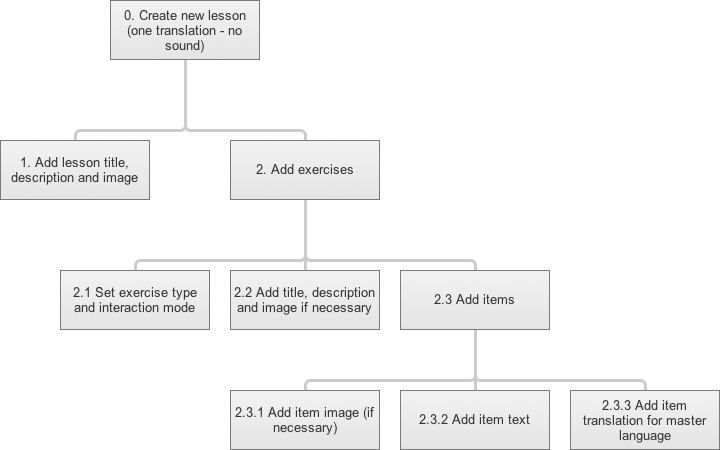
\includegraphics[width=12cm]{images/task-analysis/create_lesson}
 \caption{The tasks involved in creating a new lesson}
 \label{fig:build}
\end{figure}

%\subsubsection{Overview}
%On a high-level scale creating a new lesson or course seems rather simple. Figure \ref{fig:build} visualizes this fact. A new lesson is created within an existing or a new course and then a number of exercises are added. These exercises themselves hold a number of items, representing words or sentences.

%\subsubsection{Creating a New Course/Lesson Decomposed}
%The decomposed tasks now provide a more detailed picture of which subtasks are needed in order to actually create a new lesson. This diagram goes down to the single interactions the user needs to perform in order to reach his or her goal. It is so detailed that it could be used as a how-to-guide for someone who has not used the system before.

\subsubsection{Task 2: Localization of a Lesson} \label{sec:task-localization}
Figure \ref{fig:loc-overview} visualizes the process of translating existing content into new (display) languages. A display language is the language a user chooses which defines the language of the user interface as well as the translations and explanations he gets while learning a new language. Usually the display language corresponds to the user’s mother tongue, but sometimes learners whose mother tongue is not offered on babbel.com choose English as alternative. Babbel offers 14 different learning languages right now which can be learned by using one of the 8 different display languages. This means that there are more than 100 unique language learning combinations (14*8) that need to be maintained as well as extended when new content is added to a language.

The task of localizing existing content is a joint effort of employees at Babbel and at least two different freelancers. Usually a \ac{PM} at Babbel prepares a content package (several lessons or a whole course) for translation and manages the whole process. Afterwards a freelance translator takes over and translates all the necessary content based on a time plan. When he or she has finished a package the work is handed over to a proofreader who might do some corrections or suggest improvements. Figure \ref{fig:loc-overview} presents a high-level view of the localization process.
% watch out when switching task and user analysis again the project manager appears first in the user analysis

\begin{figure}[h]
 \centering
 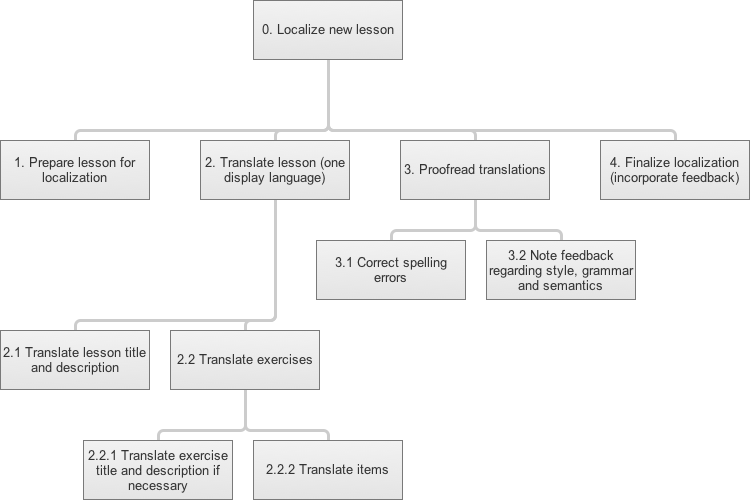
\includegraphics[width=12cm]{images/task-analysis/localize_lesson}
 \caption{Overview of Localization Process}
 \label{fig:loc-overview}
\end{figure}

%\subsubsection{Preparing a Course/Lesson for Localization Decomposed} \label{sec:preparing-loc}
%Before a course or lesson can be translated a few steps are usually necessary to ensure the translator will not encounter any problems during the process. Furthermore it needs to be ensured that end-users are not affected by making the content that is not ready yet invisible to them. This task is usually performed by a project manager.

%\subsubsection{Translation of a Course/Lesson Decomposed}
%Once a course or lesson has been setup for translation the work is handed over to a translator. Figure \ref{fig:loc-trans} shows which subtasks are necessary in order to translate a complete course.

%\subsubsection{Proofreading a Translation Decomposed}
%After the work of the translator is finished the proofreader gets informed. His job is to check the work of the translator for spelling errors or content-related problems. Spelling errors are corrected right away, but instances where the proofreader disagrees with a matter of style or how something is translated are noted in a Google Sheets file and discussed later on. As can be seen in figure \ref{fig:loc-proof} the proofreader only uses the content authoring tool when he or she wants to correct a spelling mistake.

%\subsubsection{Finalizing a Localization Decomposed}
%Finalization means that the translator looks at the comments of the proofreader and implements the suggestions if he or she agrees with them. If not, a discussion between translator and proofreader takes place. They try to settle the issue independently first and only if no agreement can be reached a project manager at Babbel is consulted. When all issues have been resolved the work is handed back to Babbel where the work of the freelancers is evaluated once more by a final quality assurance.

% \subsubsection{Task 3: Image Assignment}
% % still work in progress


% \subsubsection{Task 4: Sound Recording}
% Sound recording is the process of turning the different vocabulary items into speech. Only the learning language is recorded, not the translations. The recordings are done by native speakers who work as freelancers. Whenever new content is ready for recording (usually several lessons or a whole course) the speakers get informed of what exactly needs to be recorded. They can either do this at home, provided they use a high-quality microphone, or come to the Babbel offices and record in a professional studio. Either way, the tool they use, is the same. The recorded sounds end up on the media server and the sound IDs are linked to the respective items. After the speaker has finished his or her work package a full-time employee checks whether the recordings meet the quality standards and if not some sounds need to be re-recorded.

% \begin{figure}[h!]
%  \centering
%  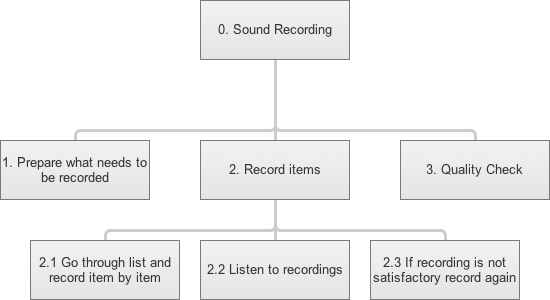
\includegraphics[width=9cm]{images/task-analysis/sound_recording}
%  \caption{Sound Recording Process}
%  \label{fig:sound-recording}
% \end{figure}

\subsubsection{Task 3: Quality Assurance} \label{sec:task-qa}
The final quality assurance happens right before new learning content is published. A Babbel employee clicks through the content in the frontend as a normal Babbel user would. This is done in order to check whether the content works as expected and the application does not break down at some point because a bug has been introduced. It is also the last chance of spotting spelling or grammar mistakes or checking whether the content complies with different conventions and has a consistent style.

\begin{figure}[h]
 \centering
 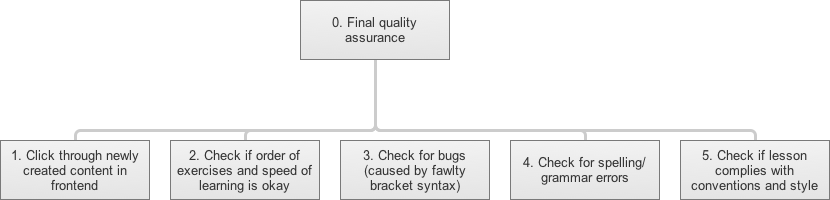
\includegraphics[width=\textwidth]{images/task-analysis/quality_assurance}
 \caption{Quality Assurance Process}
 \label{fig:qa-process}
\end{figure}

\subsection{Conclusion}
The analysis made a few things obvious. First of all, collaborating and communicating with colleagues is a reoccurring theme throughout most tasks. Not only the content creation process is divided between different user groups, but also some tasks themselves. For example, when a lesson is localized, there are at least three different individuals working together (project manager, translator, proofreader), who also need to communicate in some way. Right now, email and Google Sheets are used extensively for that, but it is conceivable that at least some of this communication could be facilitated by the new version control system. This could possibly speed up the whole process and streamline collaboration.

%The preparation of localizations (Figure \ref{fig:loc-overview}) is a good example of a step that could almost completely be avoided with a better interface design. Right now everything needs to be prepared and set up initially to make sure that translators only work on the content they are supposed to work on. In future, when a version control system is in place, it is imaginable to skip this process, because work will not be performed on live data anymore and reversibility of changes will be simpler.

In general, version control features could potentially ease collaboration and allow full-time employees to give freelancers more freedom in their work, because the risk of breaking live content will be lower. Furthermore, a feature similar to Github's \textit{pull request} could help to formalize the quality checks that happen throughout the process and provide a platform for communication between freelancers and full-time employees.
